
%(BEGIN_QUESTION)
% Copyright 2012, Tony R. Kuphaldt, released under the Creative Commons Attribution License (v 1.0)
% This means you may do almost anything with this work of mine, so long as you give me proper credit

Suppose an NDIR gas analyzer is proposed for measuring the concentration of nitrogen dioxide (NO$_{2}$) gas in a stream containing a high percentage of ammonia (NH$_{3}$) gas.  The infrared spectra of these two gases are shown below:

$$\includegraphics[width=15.5cm]{i01125x01.eps}$$

Identify the gases that should fill each of the cells in this NDIR analyzer:

\vskip 10pt

\begin{itemize}
\item{} Reference cell: \underbar{\hskip 50pt} gas
\vskip 10pt
\item{} Luft detector cells: \underbar{\hskip 50pt} gas
\vskip 10pt
\item{} Filter cells: \underbar{\hskip 50pt} gas {\it or} not necessary at all?
\end{itemize}

\vskip 10pt

If you have reason to believe that the proposed measurement scenario is \underbar{impossible} given these spectra, explain why you think so.


\underbar{file i01125}
%(END_QUESTION)





%(BEGIN_ANSWER)

This measurement scenario is {\bf impossible} for an NDIR analyzer, because the absorption spectrum of the interfering gas (ammonia) completely covers the absorption spectrum of the gas of interest (nitrogen dioxide).  10 point all-or-nothing!

%(END_ANSWER)





%(BEGIN_NOTES)

{\bf This question is intended for exams only and not worksheets!}.

%(END_NOTES)


